\chapter{Modellbeschreibung}\label{Modellbeschreibung}
\section{Erzeuger}
\subsection{Windenergie}
\subsection{Photovoltaik}
\section{Verbraucher}
\section{Speicher}\label{Speicher}
In diesem Abschnitt soll der Aufbau und die Steuerung der Speichermodelle erläutert werden.
Dazu werden zunächst verschiedene Batteriemodelle eingeführt und anschließend der gewählte Aufbau für
unsere Simulationen gezeigt. 
Zusätzlich soll die Umsetzung der in Abschnitt~\ref{Betriebsstrategien} angeführten Betriebsstrategien 
beschrieben werden.

\subsection{Batteriemodelle}\label{Batteriemodelle}
Batteriemodelle können grundlegend in 
\begin{itemize}
    \item mathematisch, empirische Black-Box-Modelle,
    \item elektrische Modelle und
    \item physikalisch-chemische Modelle
\end{itemize}
unterteilt werden. 
Innerhalb dieser Kategorien gibt es zusätzlich erhebliche Unterschiede in Bezug auf die Komplexität des Modells.
Die mathematischen Modelle versuchen dabei, das Verhalten von Batterien durch Umsetzung von empirisch bestimmten
Zusammenhängen abzubilden.
So können aus festgelegten Kennparamatern in Verbindung mit Eingangsgrößen die jeweiligen Ausgangsgrößen berechnet werden.
Dabei unterscheiden sich die verschiedenen Modellvarianten stark in ihrer Betrachtung einzelner Aspekte.

In der Kategorie der elektrischen Batteriemodelle wird versucht das Verhalten von Batterien durch Ersatzschaltkreise
mit einfachen elektrischen Bauteilen nachzubilden.
Auch hierbei gibt es große Unterschiede im detailgrad der einzelnen Umsetzungen, es besteht aber die Möglichkeit
auch komplexe elektrochemische Effekte zu modellieren.

Zuletzt bilden die physikalisch-chemischen Modelle wohl die aufwändigste Form.
Durch sie wird versucht auch das Zusammenspiel der einzelnen Materialien innerhalb der Batterie nachzubilden.
Dadurch kann das Verhalten einzelner Batteriezellen sehr genau untersucht werden, in der Praxis sind diese
Modelle aber eher selten zu finden, da die Zusammenhänge auf einer so detaillierten Ebene nur schwer zu ermitteln sind
und Simulationen eher auf das Gesamtverhalten von Batteriesystemen abzielen~\parencite[]{keil2012aufbau}.

Für unsere Simulationen haben wir uns für ein mathematisches Black-Box-Modell entschieden, dass es uns ermöglicht
die Spannung, Leistung und den SOC des Batteriemodells zu betrachten.
Auf Grund der vereinfachten Umsetzung und der insgesamt trotzdem hohen Komplexität des gesamten Simulationsmodells
sollte so die Simulationsdauer möglichst gering gehalten werden.

\begin{figure}[h!]
    \centering
    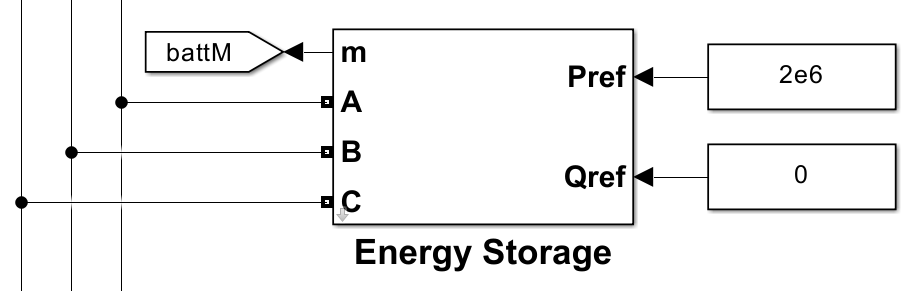
\includegraphics[width=8cm]{Abbildungen/BatterieBlackBox.png}
    \caption{Subsystem-Baustein der Batterie in Simulink}\label{BatModell}
\end{figure}
Abbildung \ref{BatModell} zeigt den Batterie-Block mit den Eingängen zur Wirk- und Blindleistung und den 
Ausgängen für jede Spannungsphase sowie dem Ausgang der Messgrößen.

\begin{figure}[h!]
    \centering
    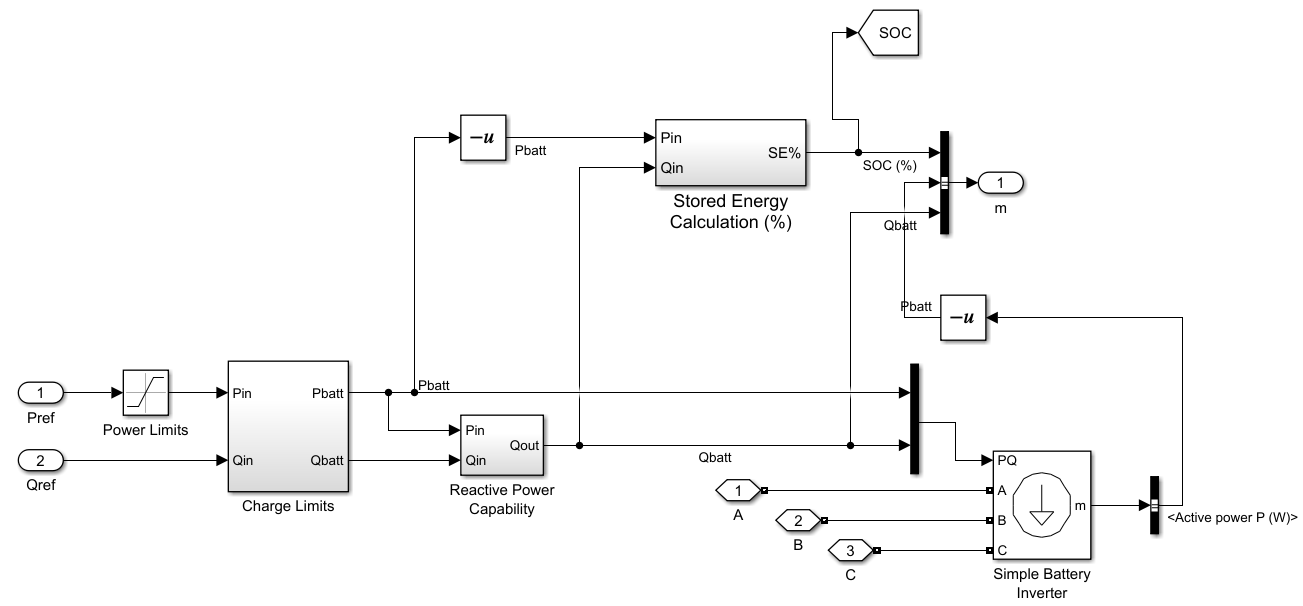
\includegraphics[width=14cm]{Abbildungen/Speicher Ebene1.png}
    \caption{Inhalt des Batteriesubsystems in Simulink}\label{BatModell1}
\end{figure}

Der Aufbau des Subsystems ist in Abbildung \ref{BatModell1} gezeigt.
Im Wesentlichen besteht das Modell aus einem Block zur Steuerung und Umsetzung der Betriebsstrategien, einem Block
zur Berechnung des SOCs und einer dreiphasigen Last die für dieses Modell als einfacher Umrichter genutzt wird.
Thermische Effekte, Verzögerungen oder Nicht-linearitäten wurden beim Entwurf dieses Modells gänzlich vernachlässigt.
Auch Selbstentladungseffekte oder Aussagen über die Lebensdauer des Batteriespeichers können mit diesem Modell nicht 
betrachtet werden.

Zur Auswertung der Betriebsstrategien und zum groben Entwurf eines realistischen Inselnetzes sollte die Komplexität
des Modells dennoch genügen.
Trotz dieser starken Vereinfachungen laufen Simulationen im dreiphasigen Modell fast in Echtzeit ab.


\subsection{Umsetzung Lade- und Entladestrategien}\label{Lade- und Entlade}

\section{Netzmodell}
\subsection{Bilanziell}
\subsection{Dreiphasig}


\chapter{Simulationsergebnisse}

\chapter{Auswertung}